%++++++++++++++++++++++++++++++++++++++++
% Don't modify this section unless you know what you're doing!
\documentclass[letterpaper,12pt]{article}
\usepackage{tabularx} % extra features for tabular environment
\usepackage{amsmath}  % improve math presentation
\usepackage{graphicx} % takes care of graphic including machinery
\usepackage[margin=1in,letterpaper]{geometry} % decreases margins
\usepackage{cite} % takes care of citations
\usepackage[final]{hyperref} % adds hyper links inside the generated pdf file
\usepackage{pgfplotstable, booktabs}
\usepackage{placeins}
\usepackage{tabularray}
\usepackage{titlesec}
\usepackage{fancyhdr}
\usepackage{empheq}
\usepackage{amssymb}
\usepackage{sectsty}
\usepackage{tcolorbox}
\usepackage{listings}
\usepackage{xcolor}
\usepackage{parskip}
\usepackage{cancel}
\usepackage{enumitem}
\usepackage{amsmath}
\usepackage{mathrsfs}
\usepackage{physics}

\definecolor{codegreen}{rgb}{0,0.6,0}
\definecolor{codegray}{rgb}{0.5,0.5,0.5}
\definecolor{codepurple}{rgb}{0.58,0,0.82}

\lstdefinestyle{mystyle}{
    commentstyle=\color{codegreen},
    keywordstyle=\color{codepurple},
    numberstyle=\tiny\color{codegray},
    stringstyle=\color{codegreen},
    basicstyle=\ttfamily\small,
    breakatwhitespace=false,         
    breaklines=true,                 
    captionpos=b,                    
    keepspaces=true,                                                     
    showspaces=false,                
    showstringspaces=false,
    showtabs=false,                  
    tabsize=4
}

\lstset{style=mystyle}
  
\newcommand*\widefbox[1]{\fbox{\hspace{0em}#1\hspace{0em}}}

\pagestyle{fancy}
\fancyhf{} % Clear all header and footer fields
\fancyhead[L]{MEC E 420}
%\fancyhead[C]{Center Header}
\fancyhead[C]{Formula Sheet}
\fancyhead[R]{Alex Diep}

\fancyfoot[C]{\thepage}

\pgfplotsset{compat=1.18} 
\titleformat*{\section}{\Large\bfseries}
\titleformat*{\subsection}{\large\bfseries}

% \renewcommand{\thesection}{Question \arabic{section}}
% \renewcommand{\thesubsection}{(\alph{subsection})}
% \renewcommand*{\arraystretch}{1.5}

\hypersetup{
	colorlinks=true,       % false: boxed links; true: colored links
	linkcolor=blue,        % color of internal links
	citecolor=blue,        % color of links to bibliography
	filecolor=magenta,     % color of file links
	urlcolor=blue         
}
%++++++++++++++++++++++++++++++++++++++++
\begin{document}
\section{State Models}
Consider a system with 
\begin{enumerate}
    \item $n$, the order of the ODE 
    \item $m$, the number of inputs
    \item $p$, the number of outputs
\end{enumerate}

General procedure:
\begin{enumerate}
    \item Create $n$ state variables
    \item Create $n$ first order ODEs
    \item Write $\dot{x} = f(x, u)$
    \item Write $y = h(x, u)$
\end{enumerate}

If the system is linear, then the state model is
\begin{align*}
    \dot{x} &= Ax + Bu \\
    y &= Cx + Du
\end{align*}

\section{Numerical Simulation with MATLAB}
Example, some random order 4 system with $x_{1}(0) = 1$, $x_{2}(0) = 2$,
$u_1 = \cos(t)$, $u_2 = \sin(t)$.
\begin{lstlisting}[language=Matlab]
    function x_dot = f(t, x)
    x_dot = [
        x(3);
        x(4);
        -10*x(1) + 10*x(2) + cos(t)
        10*x(1) - 10*x(2) - sin(t)
    ];
end

[t, x] = ode45(@f, [0, 10], [1, 2, 0, 0]);
\end{lstlisting}

\section{Linearization}
Select a point $(x_0, u_0)$ and to be the equilibrium point. That is,
\begin{align*}
    f(x_0, u_0) &= 0 \\
\end{align*}

From the set of equilibrium points, choose the appropriate one to linearize about.
Then,
\begin{align*}
    A = \frac{\partial f}{\partial x} \bigg|_{x=x_0, u=u_0} \\
    B = \frac{\partial f}{\partial u} \bigg|_{x=x_0, u=u_0} \\
    C = \frac{\partial h}{\partial x} \bigg|_{x=x_0, u=u_0} \\
    D = \frac{\partial h}{\partial u} \bigg|_{x=x_0, u=u_0} \\
\end{align*}

Example for inverted pendulum on a cart with equilibrium point $x_0 = (x_10, 0,
0, 0)$ and $u_0 = 0$.
\begin{lstlisting}[language=Matlab]
% Declare symbolic variables
syms x1 x2 x3 x4 u

% Define the system
f = [
    x3;
    x4;
    (4*x4^2*sin(x2) - 3*cos(x2)*sin(x2) + 4*u)/(4 - 3*cos(x2)^2);
    (-3*x4^2*sin(x2)*cos(x2) + 3*sin(x2) -3*u*cos(x2))/(4 - 3*cos(x2)^2);
];
h = [x1; x2];

% Compute the Jacobian
dfdx = jacobian(f, [x1, x2, x3, x4])
dfdu = jacobian(f, u)
dhdx = jacobian(h, [x1, x2, x3, x4])
dhdu = jacobian(h, u)

A = subs(dfdx, [x1, x2, x3, x4, u], [x10, 0, 0, 0, 0])
B = subs(dfdu, [x1, x2, x3, x4, u], [x10, 0, 0, 0, 0])
C = subs(dhdx, [x1, x2, x3, x4, u], [x10, 0, 0, 0, 0])
D = subs(dhdu, [x1, x2, x3, x4, u], [x10, 0, 0, 0, 0])
\end{lstlisting}

\section{Solutions to Linear Systems}
Split the system into two parts: the zero-input response and the zero-state
response. 
\begin{align*}
    x(t) &= x_{\text{z-i}}(t) + x_{\text{z-s}}(t) \\
    y(t) &= C x_{\text{z-i}}(t) + C x_{\text{z-s}}(t) + Du(t)
\end{align*}

\subsection{Zero-Input Response}
The zero-input problem is:
\begin{align*}
    \dot{x} &= Ax \\
    y &= Cx\\ 
    x(0) &= x_0 \\
    u &= 0
\end{align*}

The solution is
\begin{align*}
    x_{\text{z-i}}(t) = e^{At}x_0 \\
    y_{\text{z-i}}(t) = Ce^{At}x_0
\end{align*}


\subsection{Matrix exponential properties}
\begin{gather*}
    e^{At} = \sum_{k=0}^{\infty} \frac{A^kt^k}{k!} \\
    e^{At}|_{t=0} = I \\
    e^{At_1}e^{At_2} = e^{A(t_1 + t_2)} \\
    e^{A_1t}e^{A_2t} = e^{(A_1 + A_2)t} \iff A_1A_2 = A_2A_1 \\
    (e^{At})^{-1} = e^{-At} \\
    Ae^{At} = e^{At}A \\
    \frac{d}{dt}e^{At} = Ae^{At} = e^{At}A \\
    e^{At} = Ve^{Dt}V^{-1}  = \mathcal{L}^{-1}\{sI - A\}^{-1}
\end{gather*}

\subsection{Zero-State Response}
The zero-state problem is:
\begin{align*}
    \dot{x} &= Ax + Bu \\
    y &= Cx + Du \\
    x(0) &= 0 \\
    u &= u(t)
\end{align*}

By integrating factor method, the solution is:
\begin{align*}
    x_{\text{z-s}}(t) &= \int_{0}^{t} e^{A(t-\tau)}Bu(\tau) d\tau \\
    y_{\text{z-s}}(t) &= \int_{0}^{t} Ce^{A(t-\tau)}Bu(\tau) d\tau + Du(t)
\end{align*}

\subsection{Total Response}
The total trajectory and response respectively are:
\begin{align*}
    x(t) &= \underbrace{e^{At}x_0}_{x_{\text{z-i}}(t)} + \underbrace{\int_{0}^{t} e^{A(t-\tau)}Bu(\tau) d\tau}_{x_{\text{z-s}}(t)} \\
    y(t) &= \underbrace{Ce^{At}x_0}_{y_{\text{z-i}}(t)} + \underbrace{\int_{0}^{t} Ce^{A(t-\tau)}Bu(\tau) d\tau + Du(t)}_{y_{\text{z-s}}(t)}
\end{align*}

\section{Laplace Transform Method}
\subsection{Laplace Transform and Properties}
\begin{align*}
    \mathcal{L}{f(t)} &= F(s) = \int_{0}^{\infty} f(t)e^{-st} dt \\
    \mathcal{L}{\dot{f}(t)} &= sF(s) - f(0) \\
    \mathcal{L}{\ddot{f}(t)} &= s^2F(s) - sf(0) - \dot{f}(0) \\
    \mathcal{L}\left\{\int_{0}^{t} f(\tau) d\tau\right\} &= \frac{F(s)}{s} \\
    \mathcal{L}{f(t-t_d)} &= e^{-st_d}F(s) \\
\end{align*}

\subsection{Poles and Convergence}
\begin{itemize}
    \item In general, the right most pole determines the region of convergence. 
    \item Use the analogy that the real part of poles correspond to the expontential decay rate of the system and the imaginary part corresponds to the oscillation frequency.
    \item Repeated poles is correspond to $t e^{-at}$ or $t \sin(at)$.
    \item idk i might add fvt later
\end{itemize}

\subsection{Solution to State Space Model}
The trajectory and response respectively are:
\begin{align*}
    x(t) &= \underbrace{\mathcal{L}^{-1}\{(sI - A)^{-1}x_0\}}_{x_{\text{z-i}}(t)} + \underbrace{\mathcal{L}^{-1}\{(sI - A)^{-1}BU(s)\}}_{x_{\text{z-s}}(t)} \\
    y(t) &= \underbrace{\mathcal{L}^{-1}\{C(sI - A)^{-1}x_0\}}_{y_{\text{z-i}}(t)} + \underbrace{\mathcal{L}^{-1}\{[C(sI - A)^{-1}B + D]U(s)\}}_{y_{\text{z-s}}(t)}
\end{align*}

\subsection{Transfer Function}
The transfer function is defined from:
\begin{align*}
    Y(s) &= \underbrace{C (sI - A)^{-1} x_0}_{Y_{\text{z-i}}(s)} + \underbrace{\overbrace{[C(sI - A)^{-1} B + D]}^{G(s)} U(s)}_{Y_{\text{z-s}}(s)} \\
    G(s) &= C(sI - A)^{-1}B + D
\end{align*}

\section{Step Response}
\subsection{First Order System}
The standard first-order system is described by the following transfer function:
\begin{align*}
    G(s) = \frac{K}{\tau s + 1}
\end{align*}
For a step response $u = u_{0}(t)\implies U = 1/s$, the output is:
\begin{align*}
    Y(s) &= \frac{K}{\tau s + 1} \frac{1}{s} \\
    y(t) &= K(1 - e^{-t/\tau})
\end{align*}
To find the time constant $\tau$ and the gain $K$, we can use some properties:
\begin{align*}
    \lim_{t\to\infty} y(t) = K(1 - e^{-t/\tau}) = K \\
    y(\tau) = K(1 - e^{-1}) = 0.632K = 63.2\%K
\end{align*}
\subsection{Second Order System}
The standard second-order system is described by the following transfer function:
\begin{align*}
    G(s) = \frac{\omega_n^2}{s^2 + 2\zeta\omega_n s + \omega_n^2}
\end{align*}
For a step response $u = \alpha u_{0}(t)\implies U = 1/s$, the response can be obtained
by using $\omega_d = \omega_n\sqrt{1 - \zeta^2}$:
\begin{align*}
    y(t) = \alpha - \alpha e^{-\zeta\omega_n t}\left[\cos(\omega_d t) +
     \frac{\zeta \omega_n}{\omega_d}\sin(\omega_d t)\right]
\end{align*}
To determine $\zeta$ and $\omega_n$, define overshoot $M_p = (y_{\text{max}} -
y_{\infty})/y_{\infty}$ and peak time $t_p \implies y(t_p) = y_{\text{max}}$.
\begin{align*}
    \zeta = \frac{(\ln(M_p))^2}{\pi^2 + (\ln(M_p))^2} \\
    \omega_n = \frac{\pi}{t_p\sqrt{1 - \zeta^2}}
\end{align*}
\section{Impulse Response}
Recall the Dirac delta function $\delta(t)$ is defined as:
\begin{align*}
    \int_{-\infty}^{\infty} \delta(t) dt = 1 \\
    \delta(t) = 0 \quad \forall t \neq 0 \\
    \int_{-\infty}^{\infty} f(t)\delta(t-t_0) dt = f(t_0)
\end{align*}
The zero-state response to a impulse input $u = \delta(t)$ is:
\begin{align*}
    g(t) &= \int_{0}^{t} C e^{A(t-\tau)}B \delta(\tau) d\tau + D \delta(t) \\
    = C e^{At}B + D \delta(t)
\end{align*}
The Laplace transform of the impulse response is:
\begin{align*}
    G(s) = C(sI - A)^{-1}B + D
\end{align*}
This is no coincidence. The transfer function is the Laplace transform of the
impulse response.

By convolution,
\begin{align*}
    y_{\text{z-s}}(t) &= (g * u)(t) \\
    &= \int_{0}^{t} g(t - \tau) u(\tau) d\tau \\
    &= \int_{0}^{t} C e^{A(t-\tau)}B u(\tau) d\tau + D u(t) \\
\end{align*}
Which is exactly the zero-state response obtained using the time-domain integrating
factor method.

\section{Realization}
to do later cause lazy

\section{Stability}
\subsection{Internal Stability}
Internal stability is concerned with unforced ($u=0$) systems. This corresponds to the trajectory $x_{\text{z-i}}(t)$ and the response $y_{\text{z-i}}(t)$.

For $x(0)$, the system is internally \textbf{stable} about an equilibrium point $x_e$ if and only if for every $\epsilon > 0$, there exists a $\delta > 0$ such that:
\begin{align*}
    \norm{x(0) - x_e} < \delta \implies \norm{x(t) - x_e} < \epsilon, \quad \forall t \geq 0
\end{align*}
A system is said to be \textbf{asymptotically stable} if it is stable and $\lim_{t\to\infty} x(t) = x_e$.

For linear systems, the system is internally stable if and only if every eigenvalue of $A$ has a negative real part. 
$\text{Re}(\lambda_i) < 0, \forall i = 1, \dots n$.

\subsection{BIBO Stability}
BIBO (bounded-input bounded-output) stability is concerned with zero state systems. This corresponds to the trajectory 
$x_{\text{z-s}}(t)$ and the response $y_{\text{z-s}}(t)$.

Assume $G(s)$ is a rational and proper transfer function. Then, the system is BIBO stable if and only if every pole of $G(s)$ has a 
negative real part. $\text{Re}(\text{pole}_i) < 0, \forall i = 1, \dots n$.

If the system is not stable, then there exists a bounded input $u(t)$ such that the output $y(t)$ is unbounded. Not all bounded inputs
will cause an unstable BIBO system to be unbounded.

\subsection{Connection between Internal and BIBO Stability}
For a linear system, internal stability implies BIBO stability. However, BIBO stability does not imply internal stability. This is because
the poles of $G(s)$ are a subset of the eigenvalues of $A$.

asymptotic stability $\implies$ BIBO stability
\subsection{Closed Loop Systems}
\begin{figure}[h]
    \centering
    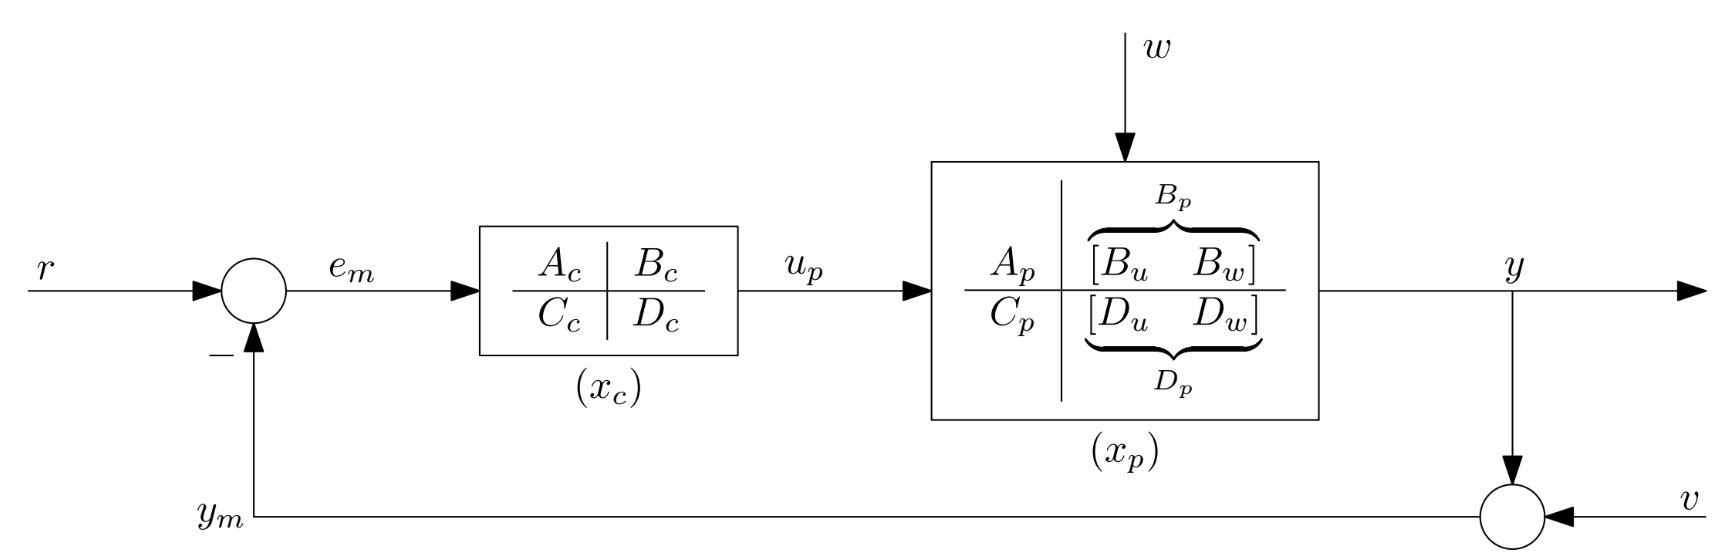
\includegraphics[width=0.5\textwidth]{closed loop diagram.png}
    \caption{Closed loop system}
\end{figure}
Assume:
\begin{itemize}
    \item Both controller ($A_c$, $B_c$, $C_c$, $D_c$) and plant ($A_p$, $B_p$, $C_p$, $D_p$) are minimal realizations.
    \item $D_c= 0$ or $D_p = [D_u, D_w] = 0$, such that $D_c D_u = D_u D_c = 0$ and $D_c D_w = D_w D_c = 0$.
\end{itemize}
Then, the state-space form of the closed loop system is:
\begin{align*}
    \dot{x}_cl &= \begin{bmatrix}
        \dot{x}_c \\
        \dot{x}_p
    \end{bmatrix} = \underbrace{
    \begin{bmatrix}
    A_c - B_c D_u C_c & -B_c C_p \\
    B_u C_c & A_p - B_u D_c C_p
    \end{bmatrix}}_{A_{cl}}
    \begin{bmatrix}
        x_c \\
        x_p
    \end{bmatrix} + \underbrace{
    \begin{bmatrix}
        B_c & -B_c D_w & -B_c \\
        B_u D_c & B_w & -B_u D_c
    \end{bmatrix}}_{B_{cl}}
    \begin{bmatrix}
        r \\
        w \\
        v 
    \end{bmatrix} \\
    y_cl &= \begin{bmatrix}
        e_m \\
        u_p \\
        y  \\
        y_m 
    \end{bmatrix} = \underbrace{
    \begin{bmatrix}
        -D_u C_c & -C_p \\
        C_c & -D_c C_p \\
        D_u C_c & C_p \\
        D_u C_c & C_p 
    \end{bmatrix}}_{C_{cl}}
    \begin{bmatrix}
        x_c \\
        x_p
    \end{bmatrix} + \underbrace{
    \begin{bmatrix}
        1 & -D_w & -1 \\
        D_c & 0 & -D_c \\
        0 & D_w & 0 \\
        0 & D_w & 1
    \end{bmatrix}}_{D_{cl}}
    \begin{bmatrix}
        r \\
        w \\
        v
    \end{bmatrix}
\end{align*}
Casting to transfer functions where
\begin{align*}
    G_c(s) &:= C_c (sI - A_c)^{-1} B_c + D_c \\
    G(s) &:= C_p (sI - A_p)^{-1} B_p + D_p := 
    \begin{bmatrix}
        G_p(s) & G_d(s)
    \end{bmatrix}
\end{align*}
Then the system becomes:
\begin{align*}
    \begin{bmatrix}
        E_m \\
        U_p \\
        Y \\
        Y_m
    \end{bmatrix}
    &=
    \begin{bmatrix}
        \frac{1}{1+G_p G_c} & \frac{G_d}{1+G_p G_c} & \frac{-1}{1+G_p G_c} \\
        \frac{G_c}{1+G_p G_c} & \frac{-G_c G_d}{1+G_p G_c} & \frac{-G_c}{1+G_p G_c} \\
        \frac{G_p G_c}{1+G_p G_c} & \frac{G_d}{1+G_p G_c} & \frac{-G_p G_c}{1+G_p G_c} \\
        \frac{G_p G_c}{1+G_p G_c} & \frac{G_d}{1+G_p G_c} & \frac{-1}{1+G_p G_c}
    \end{bmatrix}
    \begin{bmatrix}
        R \\
        W \\
        V
    \end{bmatrix}
\end{align*}
\subsection{Unmodeled Disturbance Input}
Most of the time we just assume that disturbance is added to the input $u_p$. In the transfer function matrix, $G_d = G_p$.
\subsection{Internal Stability of Closed Loop Systems}
The closed loop system is internally stable if and only if every eigenvalue of $A_{cl}$ has a negative real part.
\subsection{I/O Stability of Closed Loop Systems}
The closed loop system is I/O stable if and only if every entry of the transfer function matrix is BIBO stable. There are 
5 unique transfer functions to be considered:
\begin{align*}
    \frac{1}{1+G_p G_c} \\
    \frac{G_c}{1+G_p G_c} \\
    \frac{G_p G_c}{1+G_p G_c} \\
    \frac{G_d}{1+G_p G_c} \\
    \frac{G_c G_d}{1+G_p G_c} 
\end{align*}
If the disturbance is added to the input, then $G_d = G_p$ and then we only need to check:
\begin{align*}
    \frac{1}{1+G_p G_c} \\
    \frac{G_c}{1+G_p G_c} \\
    \frac{G_p G_c}{1+G_p G_c} \\
    \frac{G_p}{1+G_p G_c} \\
\end{align*}
\subsubsection{Characteristic Polynomial for Closed Loop Systems}
Define the numerator and denominator of the transfer functions:
\begin{align*}
    G_c := \frac{n_c}{d_c}, \quad G := [G_p, G_d] := [\frac{n_p}{d_p}, \frac{n_d}{d_d}]
\end{align*}
The characteristic polynomial is:
\begin{align*}
    P = n_p n_c + d_p d_c
\end{align*}
By \textbf{Theorem 4.4.1}, the closed loop system is I/O stable if and only if all roots of $P$ have a negative real part.

\subsubsection{Theorem 4.4.2}
The closed loop system is I/O stable if and only if
\begin{enumerate}
    \item $1 + G_p G_c$ has only negative real part roots
    \item $G_p G_c$ has no pole-zero cancellations
\end{enumerate}

\subsection{Connection Between Internal and I/O Stability}
\subsubsection{Theorem 4.4.3}
The closed loop system is internally stable if and only if it is I/O stable.
\subsubsection{Routh-Hurwitz Criterion}
The characteristic polynomial is
\begin{equation*}
    p(s) = n_p n_c + d_p d_c = s^n + a_{n-1}s^{n-1} + \dots + a_1 s + a_0, \quad a_i \in \mathbb{R}
\end{equation*}
Again, from \textbf{Theorem 4.4.1}, the closed loop system is I/O stable if and only if all roots of $P$ have a negative real part. A quick test
is 
\begin{table}[h]
    \centering
    \begin{tabular}{ll}
        p(s) & Stability Criterion \\
        \hline
        $s + a_0$ & $a_0 > 0$ \\
        $s^2 + a_1 s + a_0$ & $(\forall i) a_i > 0$ \\
        $s^3 + a_2 s^2 + a_1 s + a_0$ & $(\forall i) a_i > 0$ and $a_1 a_2 > a_0$ \\
        $s^4 + a_3 s^3 + a_2 s^2 + a_1 s + a_0$ & $(\forall i) a_i > 0$ and $a_2 a_3 > a_1$ and $(a_1 a_2 a_3 - a_{1}^2)/a_{3}^2 > a_0$
    \end{tabular}
\end{table}

\section{Graphical Methods}
\subsection{Principal of the Argument}
Theorem 5.2.1 (Principal of the Argument): Suppose $G(s)$ has no poles or zeroes on $\mathcal{D}$, but $\mathcal{D}$ encircles 
$n$ poles and $m$ zeroes of $G(s)$. Then $\mathcal{G}$ encircles the origin $n-m$ times CCW.

\subsection{Nyquist Plotting}
Input the Nyquist contour into the loop transfer function $L(s) = G_p(s) G_c(s)$ and plot the Nyquist plot. If $L(s)$ has real coefficients,
then the Nyquist plot is symmetric about the real axis.

\subsubsection{Case 1: No Poles on Re$\{s\} = 0$}
Suppose $L(s) = \frac{2}{s-1}$.
\begin{figure}[h]
    \centering
    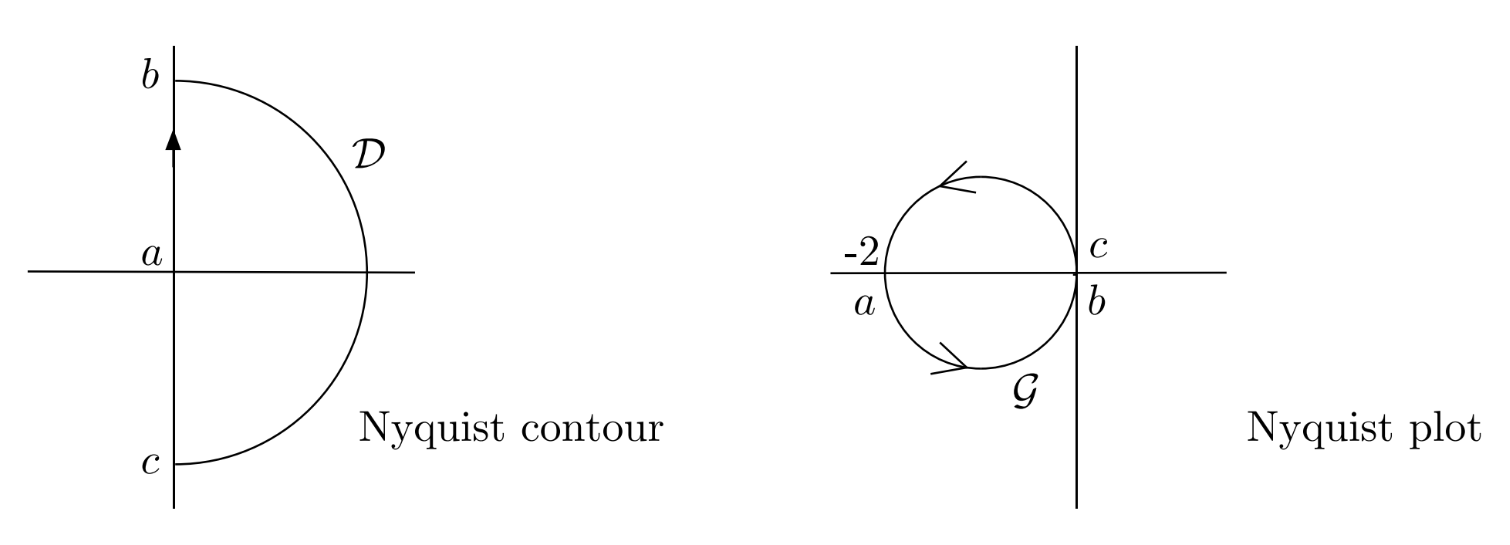
\includegraphics[width=0.5\textwidth]{case1 nyquist plots.png}
    \caption{Nyquist contour and plot for case 1}
\end{figure}
There are 2 segments to consider: $a-b$ and $b-c$. Note, by symmetry $a-b$ and $a-c$ are the same. On $a-b$, $s= j\omega$, $\omega: [0, \infty)$ 
\begin{lstlisting}[language=Matlab]
syms s 
syms omega real
L(s) = 2/(s-1);

simplify(real(L(j*omega)))
simplify(imag(L(j*omega)))
\end{lstlisting}
\begin{verbatim}
ans =
 
-2/(omega^2 + 1)
 
 
ans =
 
-(2*omega)/(omega^2 + 1)
 
>> 
\end{verbatim}
On $b-c$, $s \to \infty$. By the assumption that $L(s)$ is strictly proper, $L(s) \to 0$ as $s \to \infty$. Therefore, $b-c$ is the origin, always.

\subsubsection{Case 2: Poles on Re$\{s\} = 0$}
Suppose $L(s) = \frac{1}{s(s+1)^2}$. A right indent is required due to the $s=0$ pole. By symmetry, $c-d$ is the same as $a-b$.

\begin{figure}[h]
    \centering
    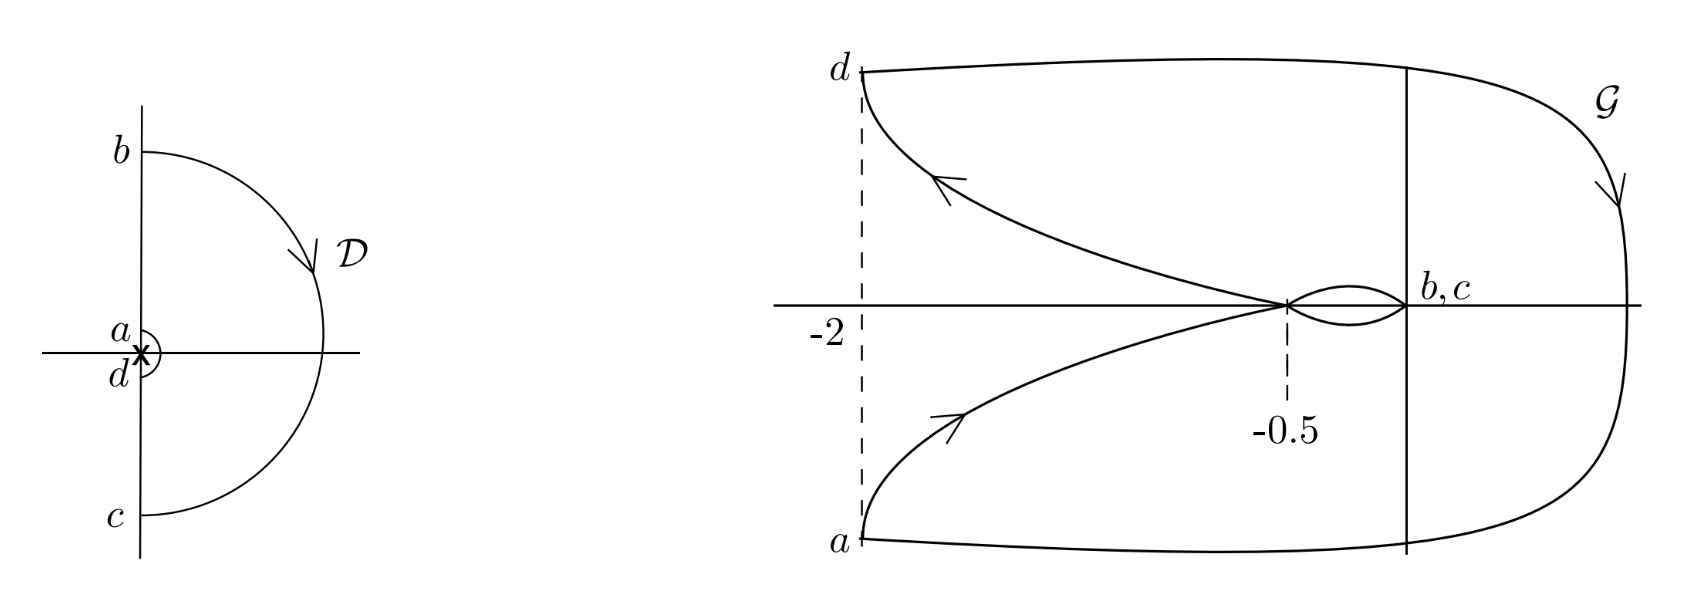
\includegraphics[width=0.5\textwidth]{case2 nyquist plots.png}
    \caption{Nyquist contour and plot for case 2}
\end{figure}

On $a-b$, $s= j\omega$, $\omega: [\epsilon, \infty)$
\begin{lstlisting}[language=Matlab]
syms s
syms omega real
L(s) = 1/(s*(s+1)^2);

simplify(real(L(j*omega)))
simplify(imag(L(j*omega)))
\end{lstlisting}
\begin{verbatim}
ans =

-2/(omega^2 + 1)^2
    
    
ans =
    
(omega^2 - 1)/(omega*(omega^2 + 1)^2)

>>
\end{verbatim}

Point $a$ is $\omega \to 0$. 

$b-c$ will go to the origin as $s \to \infty$ because $L(s)$ is strictly proper.

Lastly, for $a-d$ consider the general form $L(s)$ with a pole at $s=jy$ with multiplicity $m$. Then we can write,
\begin{align*}
    L(s) = \frac{1}{(s-jy)^m} L_1 (s)
\end{align*}
where $L_1(s)$ has no poles at $s=jy$. Then indenting at $s= jy + \epsilon e^{j\theta}$, $\epsilon \to 0$, $\theta: [-\pi/2, \pi/2]$,
\begin{align*}
    L(jy + \epsilon e^{j\theta}) = \frac{1}{\epsilon^m e^{jm\theta}} L_1(jy + \epsilon e^{j\theta}) \approx \frac{e^{-j \theta m}}{(\epsilon)^m} L_1(jy)
\end{align*}

In this case, $y = 0$ and $m = 1$. Therefore on $a-d$, 
\begin{align*}
    L(\epsilon e^{j\theta}) \approx \frac{e^{-j \theta}}{\epsilon} \left(\frac{1}{(0 + 1)^2}\right) = \frac{e^{-j \theta}}{\epsilon}
\end{align*}
This is an arc with infinite radius sweeping from $\theta: [-\pi/2, \pi/2]$ CW. 

\subsection{Nyquist Stability Criterion}
Theorem 5.3.1 (Nyquist Stability Criterion): Let $n$ denote the number of poles of $L(s) = G_p(s) G_c(s)$ in Re$\{s\} > 0$. Construct
the Nyquist plot of $L(s)$, indenting to the right around the poles around the imaginary axis. Then, the closed loop is stable 
if and only if the Nyquist plot doesn't pass through the point -1 and encircles it exactly $n$ times CCW.

\subsection{Bode Plots}
Let $G(s)=n(s)/d(s)$ be a rational transfer function. Then,$G(s)$ can be factored as a product of the following terms:
\subsubsection{Pure gain, $k$}
$G(s) = k$
If $k > 0$, 
\begin{figure}[h]
    \centering
    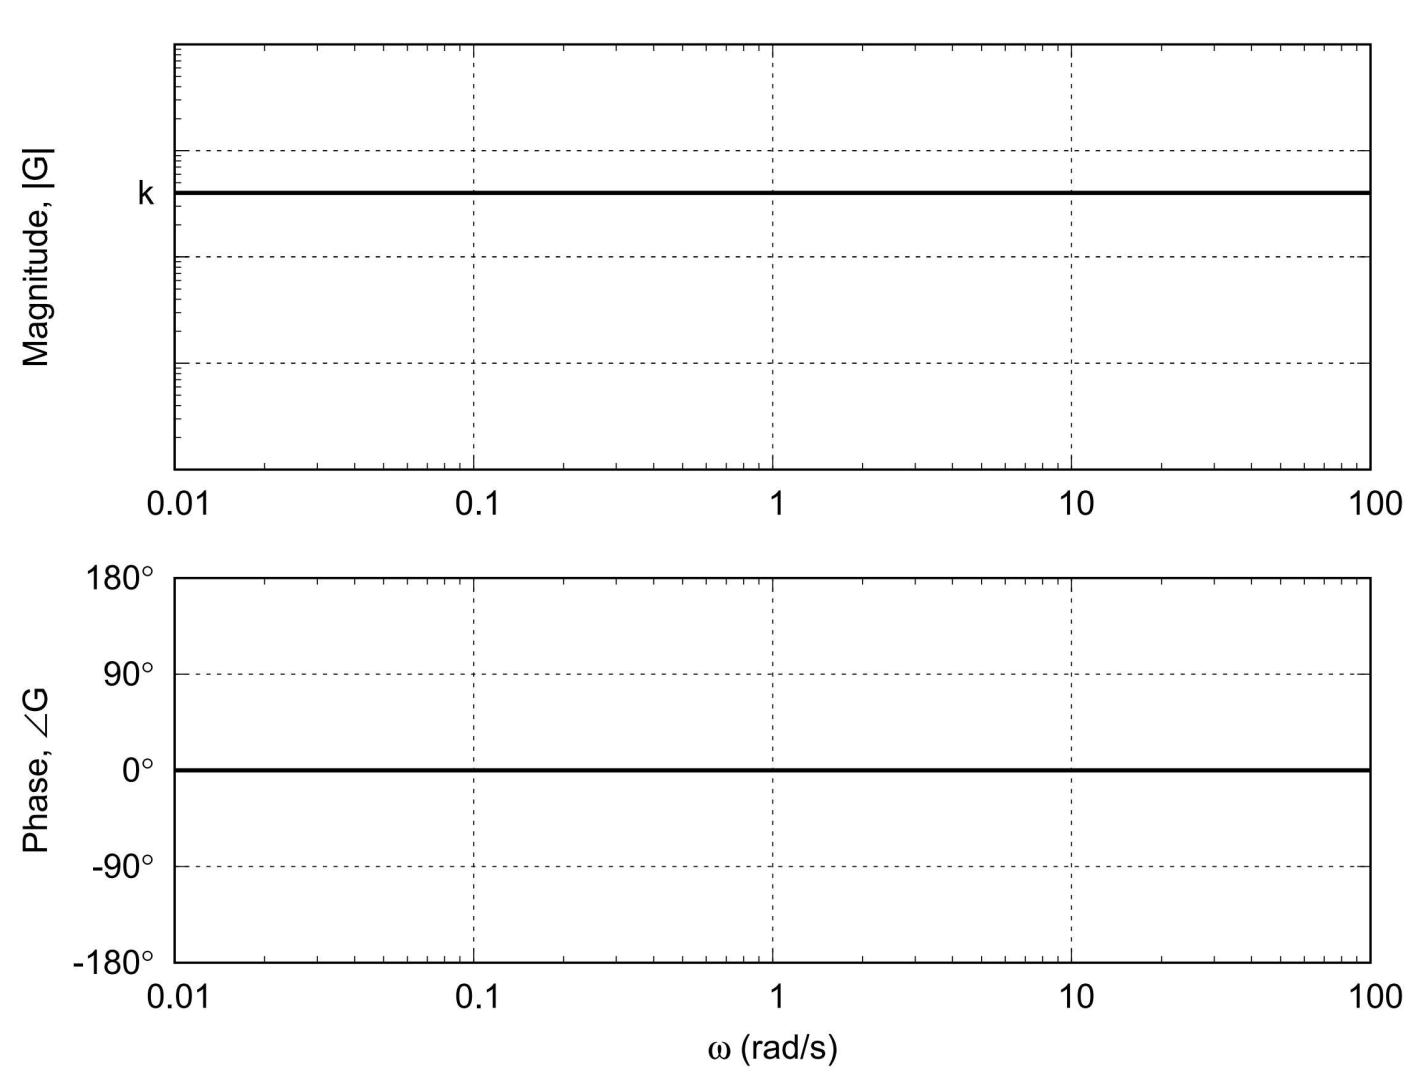
\includegraphics[width=0.6\textwidth]{case1 pure gain greater than 0.png}
    \caption{Bode plot for pure gain $k > 0$}
\end{figure}
If $k < 0$,
\begin{figure}[h]
    \centering
    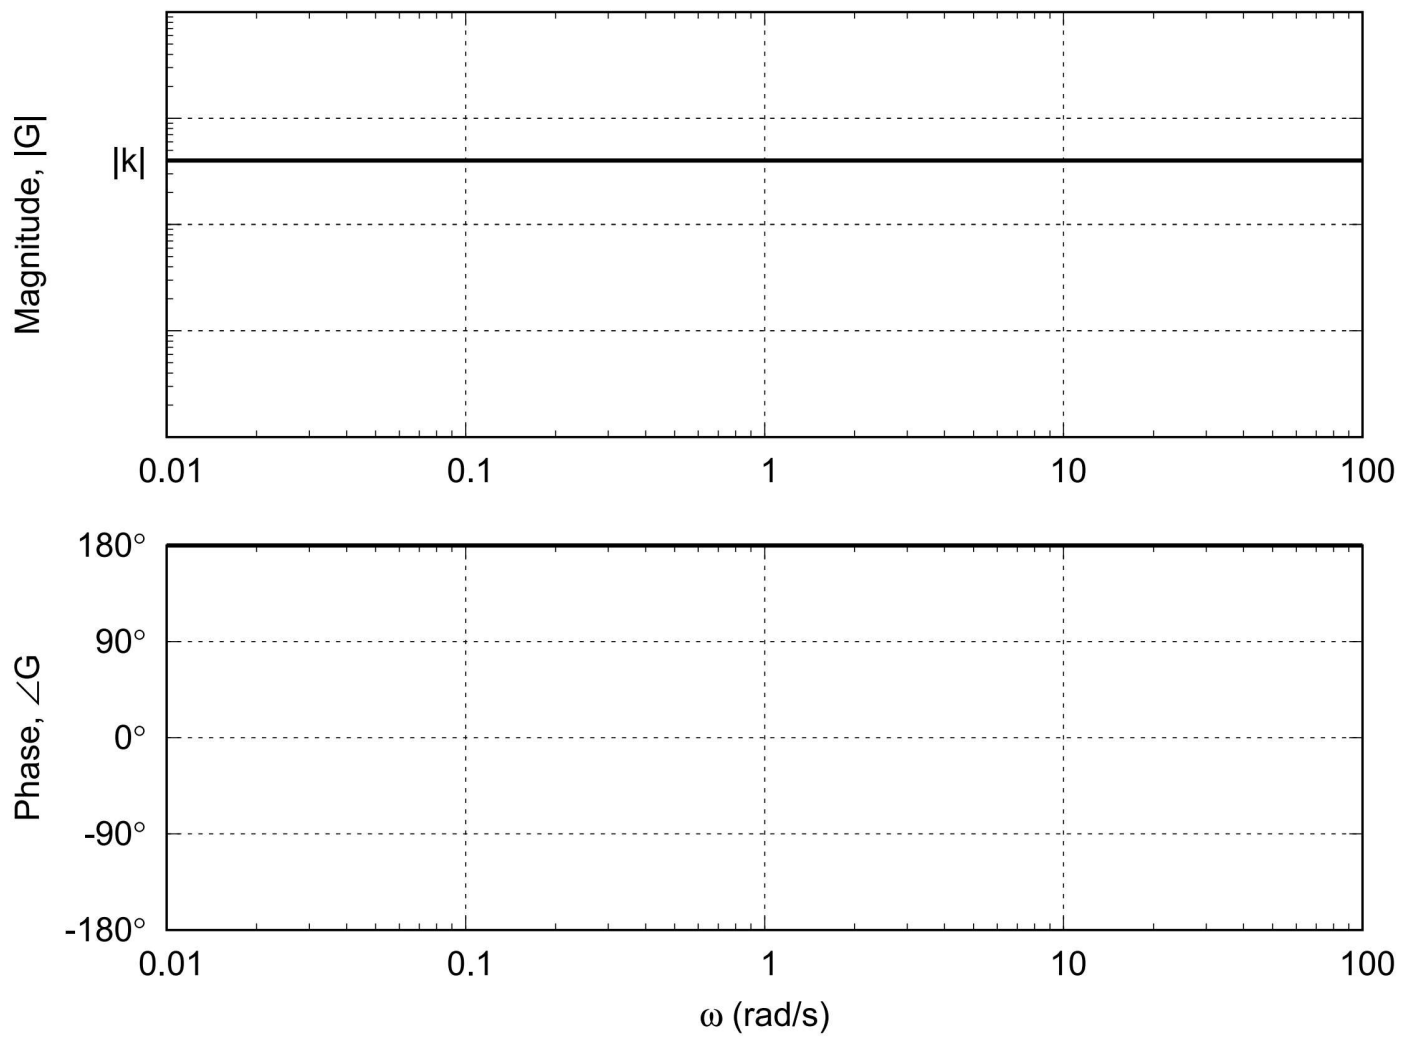
\includegraphics[width=0.6\textwidth]{case2 pure gain less than 0.png}
    \caption{Bode plot for pure gain $k < 0$}
\end{figure}
\FloatBarrier
\subsubsection{Pole or zero at the origin $G(s) = s$}
For a pole, the Bode plot is $G(j \omega) = j\omega$, $\omega \in [0, \infty)$.
\begin{figure}[h]
    \centering
    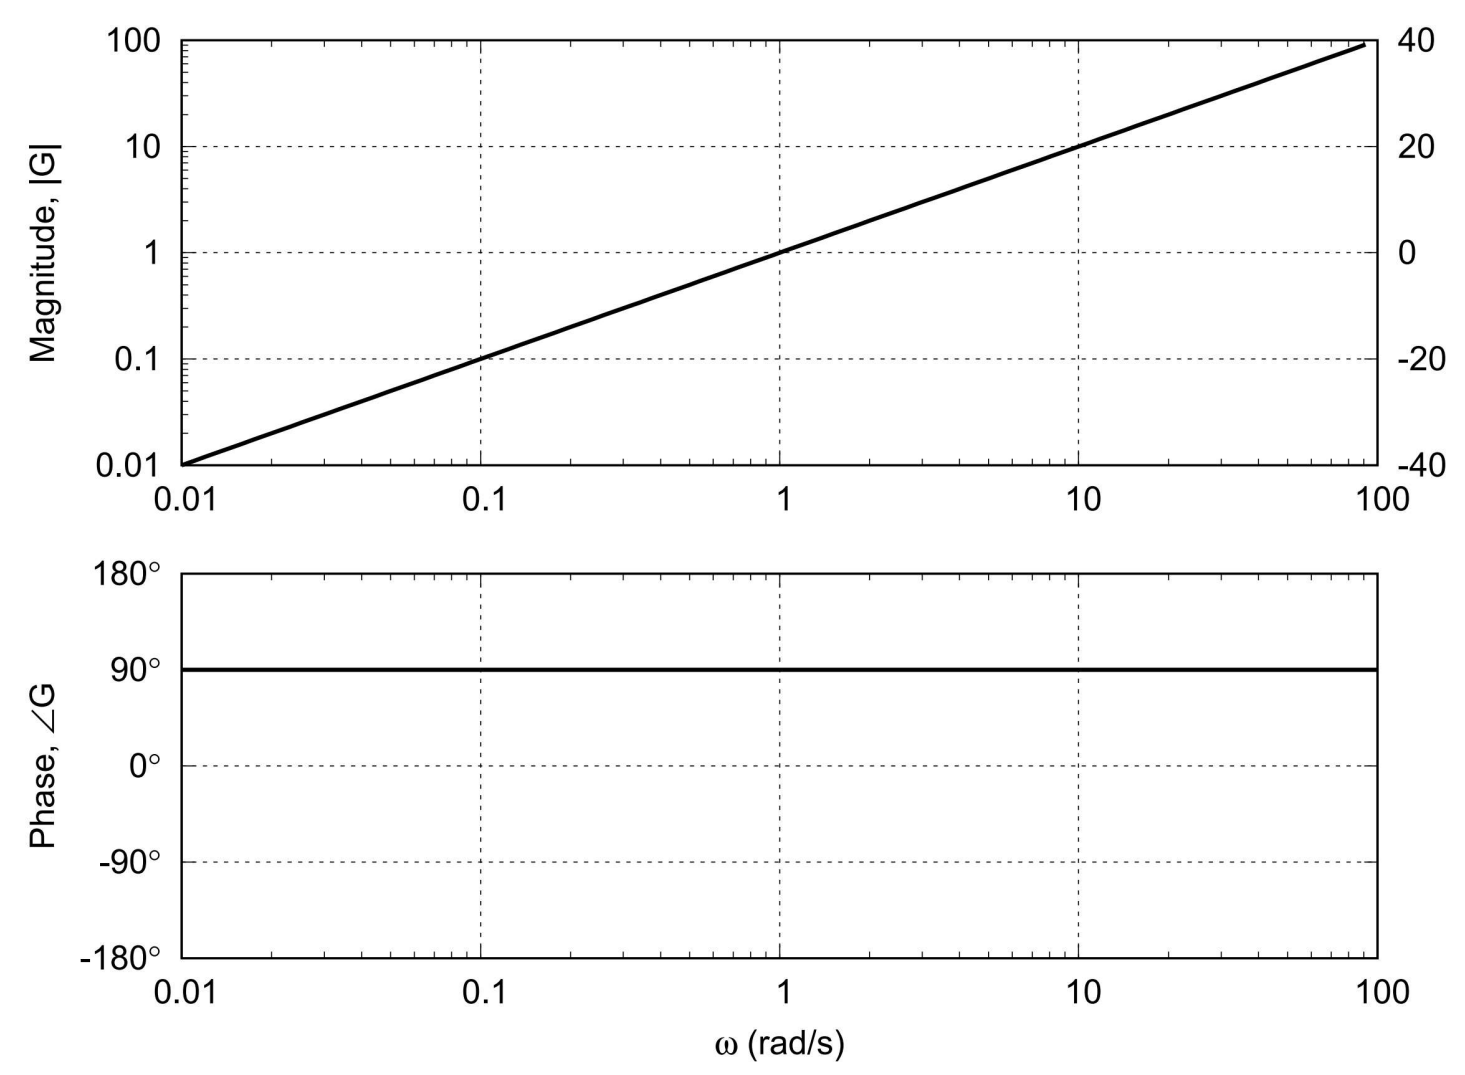
\includegraphics[width=0.6\textwidth]{case3 pole or zero at origin.png}
    \caption{Bode plot for pole at origin}
\end{figure}
\FloatBarrier

\subsubsection{Real non-zero pole or zero $G(s) = \tau s \pm 1$}
For $G(s) = \tau s + 1$, the Bode plot is $G(j \omega) = 1 + j\omega \tau$, $\omega \in [0, \infty)$.
\begin{figure}[h]
    \centering
    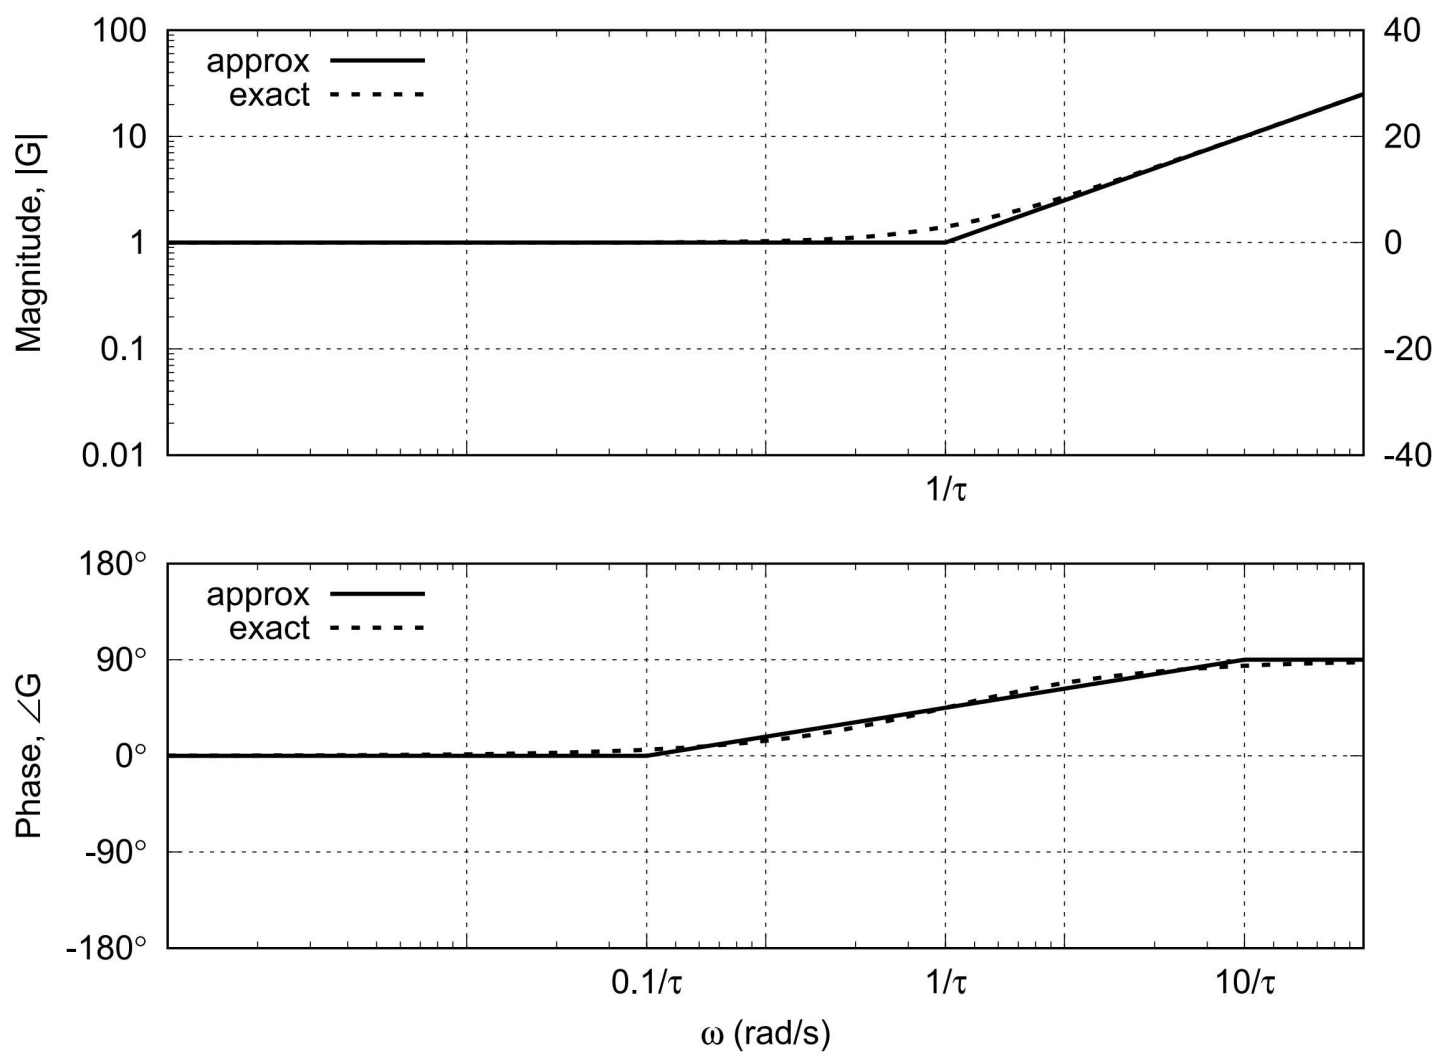
\includegraphics[width=0.6\textwidth]{case4 real nonzero root negative.png}
    \caption{Bode plot for real non-zero pole or zero $G(s) = \tau s + 1$}
\end{figure}

For $G(s) = \tau s - 1$, the Bode plot is $G(j \omega) = -1 + j\omega \tau$, $\omega \in [0, \infty)$.
\begin{figure}[h]
    \centering
    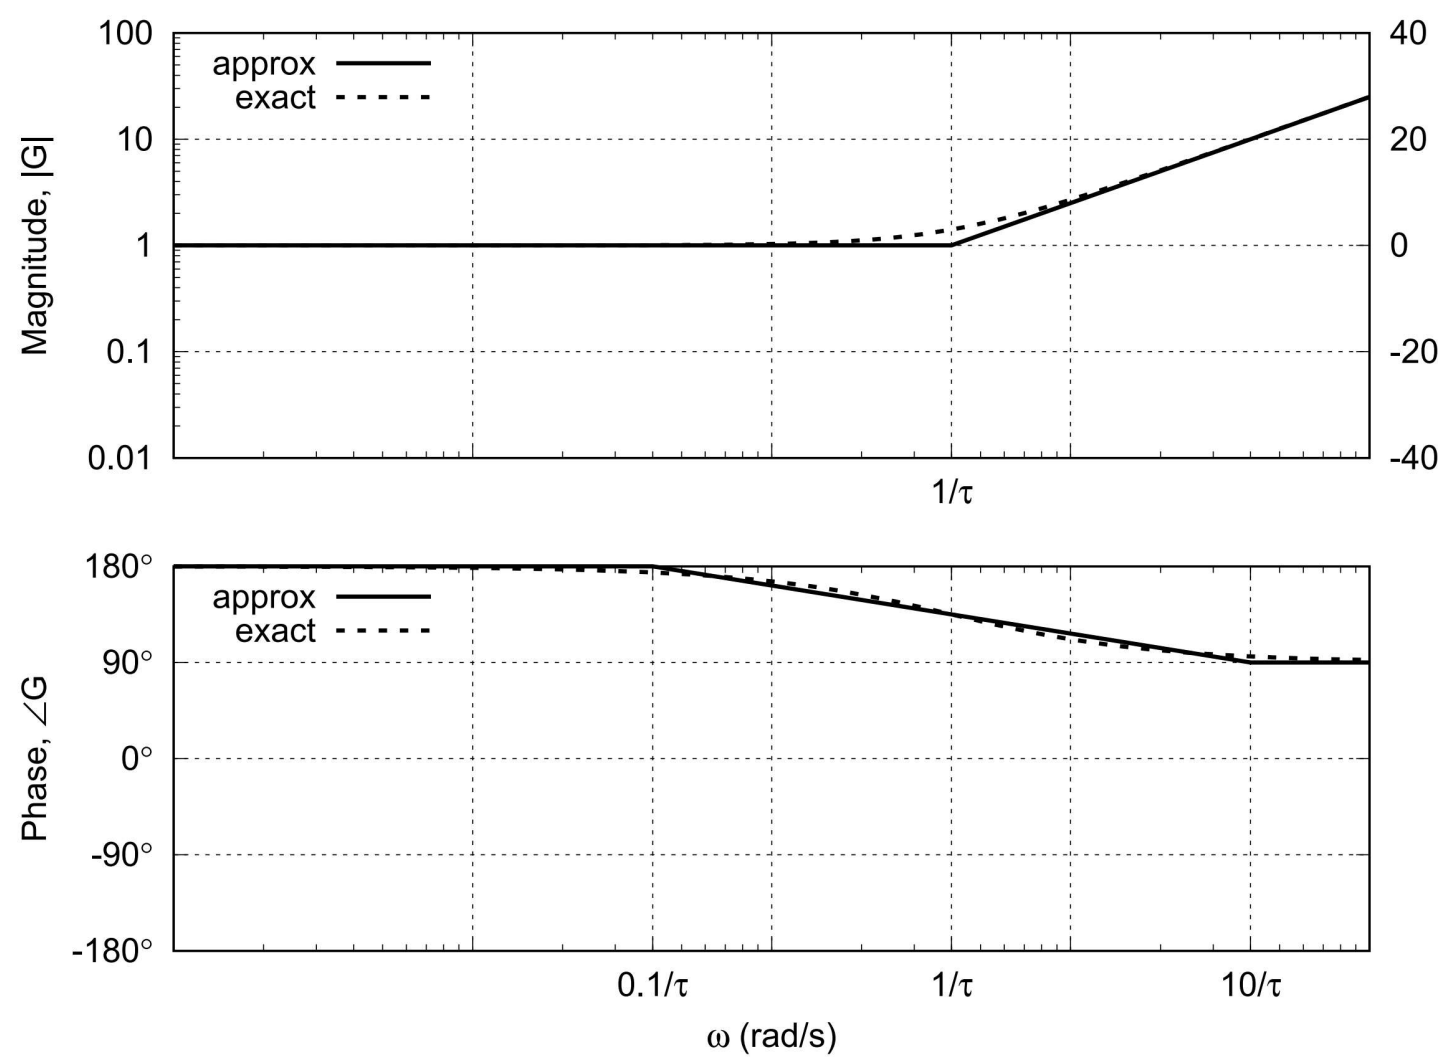
\includegraphics[width=0.6\textwidth]{case5 real nonzero root positive.png}
    \caption{Bode plot for real non-zero pole or zero $G(s) = \tau s - 1$}
\end{figure}
\FloatBarrier
\subsubsection{Complex conjugate poles or zeros $G(s) = \frac{1}{\omega_{n}^2} (s^2 + 2\zeta \omega_n s + \omega_n^2)$, $\omega_n > 0$, $\zeta \in [0, 1]$}
If the roots of $G(s)$ lie Re$\{s\} < 0$, then $G(j \omega) = \frac{1}{\omega_{n}^2} (\omega_n^2 - \omega^2 + j2\zeta \omega_n \omega)$, $\omega \in [0, \infty)$.
\begin{figure}[h]
    \centering
    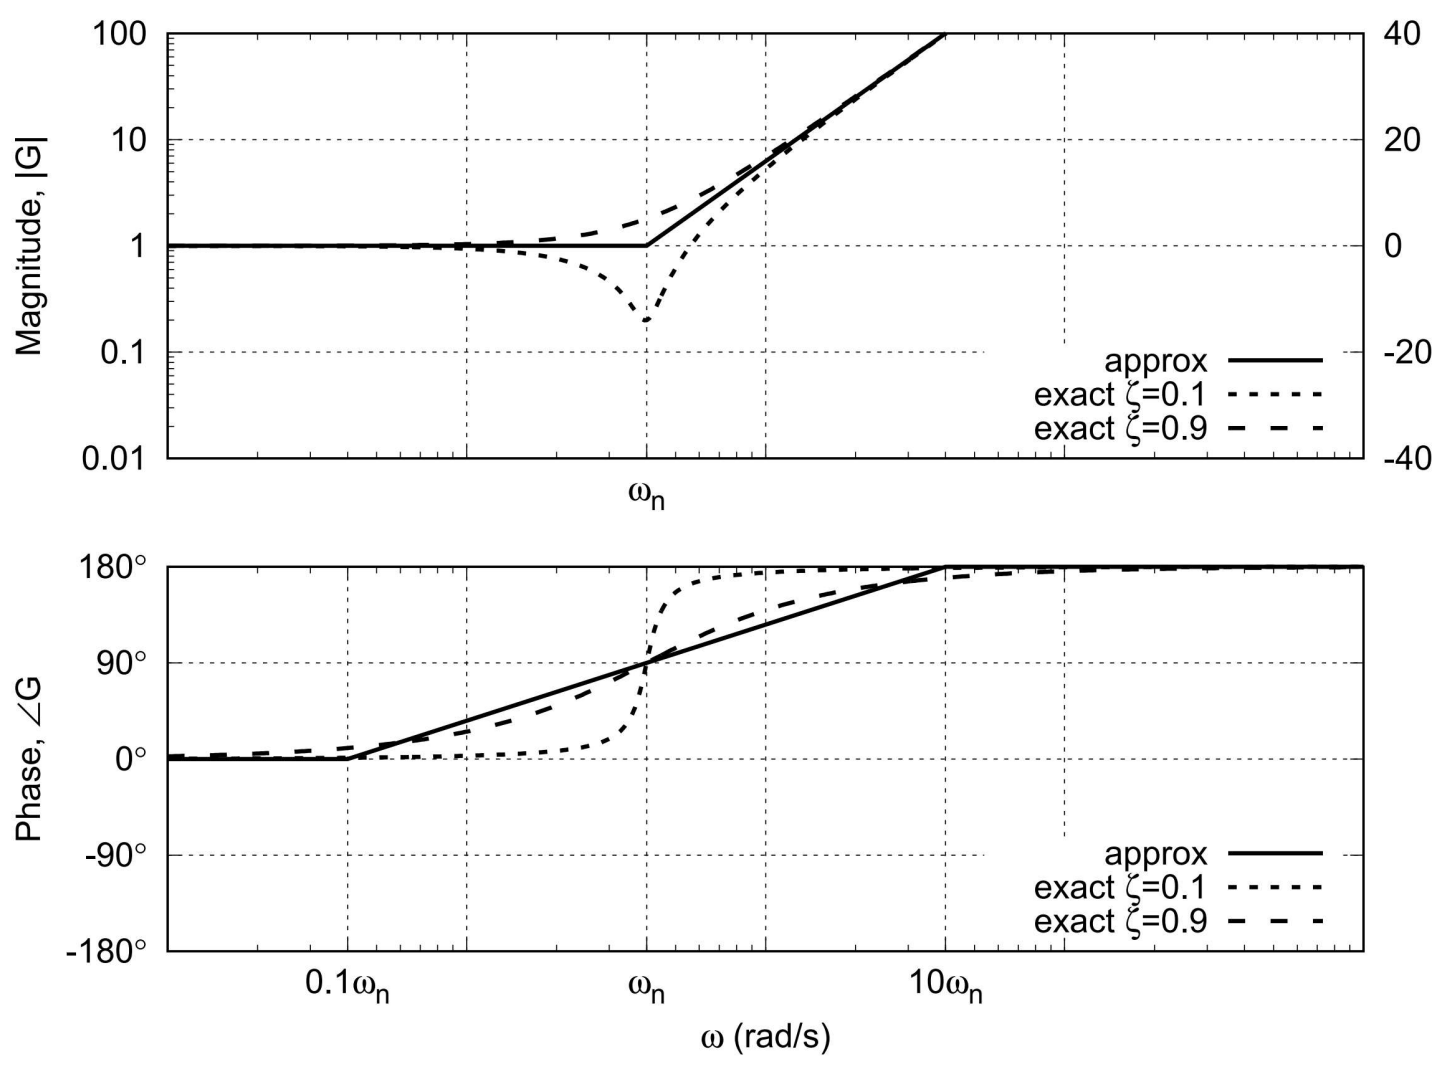
\includegraphics[width=0.6\textwidth]{case6 complex conjugate negative.png}
    \caption{Bode plot for complex conjugate with negative roots of $G(s) = \frac{1}{\omega_{n}^2} 
    (s^2 + 2\zeta \omega_n s + \omega_n^2)$, $\omega_n > 0$, $\zeta \in [0, 1]$}
\end{figure}
\FloatBarrier
If the roots of $G(s)$ lie Re$\{s\} > 0$, then $G(j \omega) = \frac{1}{\omega_{n}^2} (\omega_n^2 - \omega^2 - j2\zeta \omega_n \omega)$, $\omega \in [0, \infty)$.
\begin{figure}[h]
    \centering
    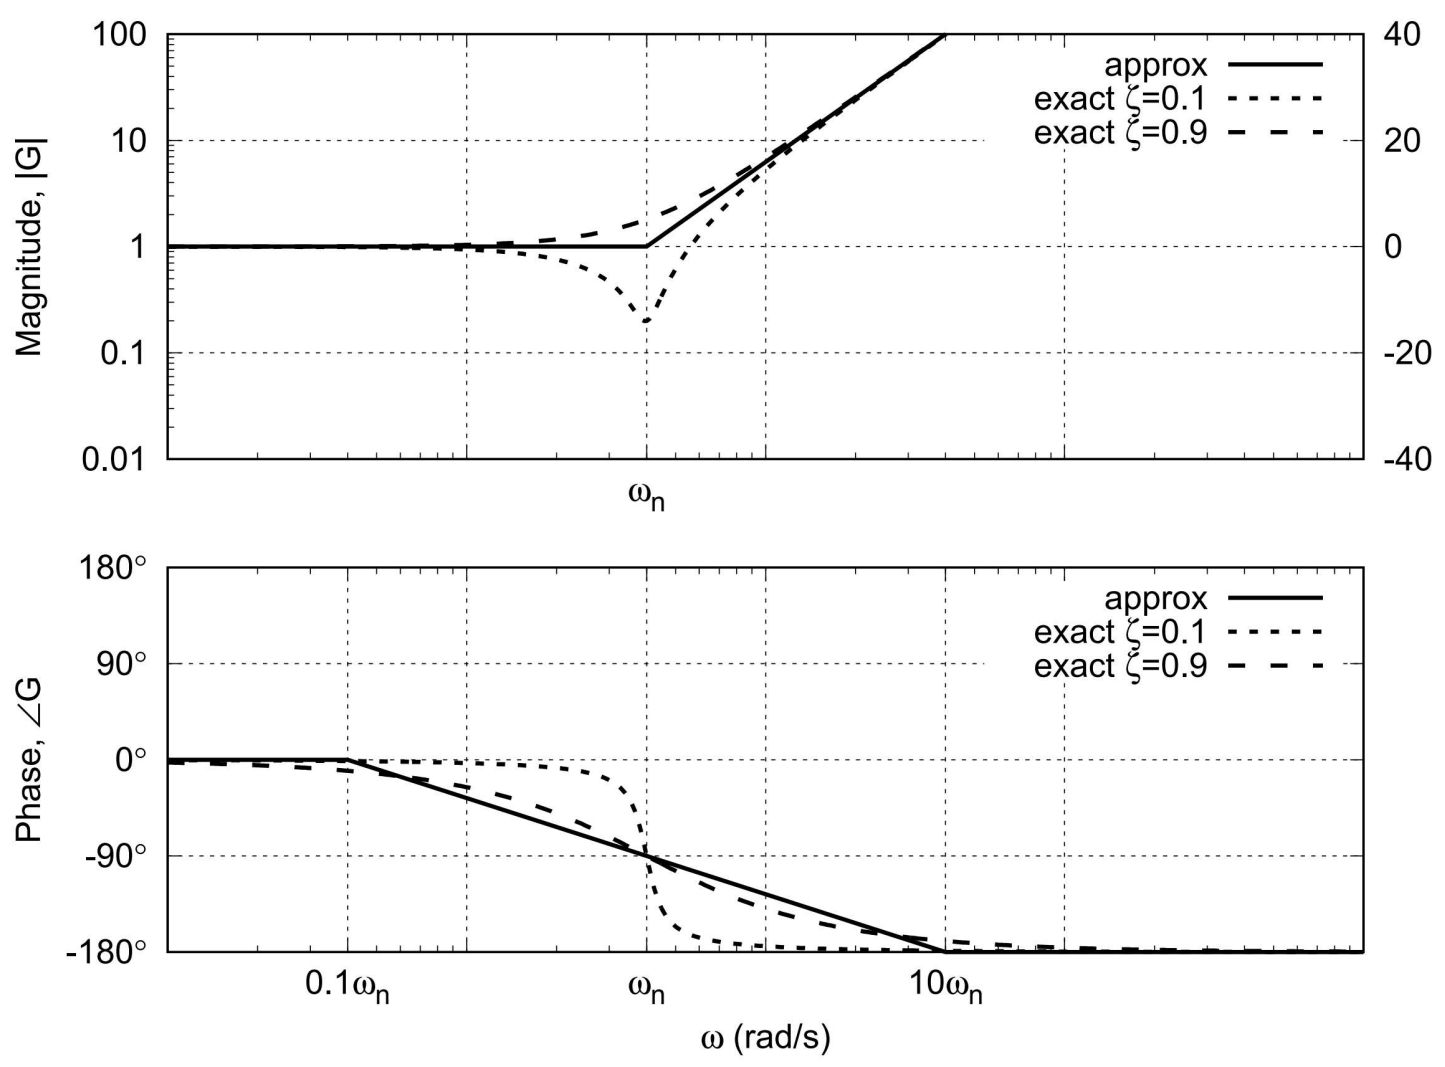
\includegraphics[width=0.6\textwidth]{case7 complex conjugate positive.png}
    \caption{Bode plot for complex conjugate with positive roots of $G(s) = \frac{1}{\omega_{n}^2} 
    (s^2 + 2\zeta \omega_n s + \omega_n^2)$, $\omega_n > 0$, $\zeta \in [0, 1]$}
\end{figure}
\FloatBarrier
The roots of $G(s)$ lie on Re$\{s\} = 0$ iff $\zeta = 0$. Then $G(s) = \frac{1}{\omega_{n}^2} (s^2 + \omega_n^2)$ and 
$G(j \omega) = \frac{1}{\omega_{n}^2} (\omega_n^2 - \omega^2)$, $\omega \in [0, \infty)$ gives 
\begin{figure}[h]
    \centering
    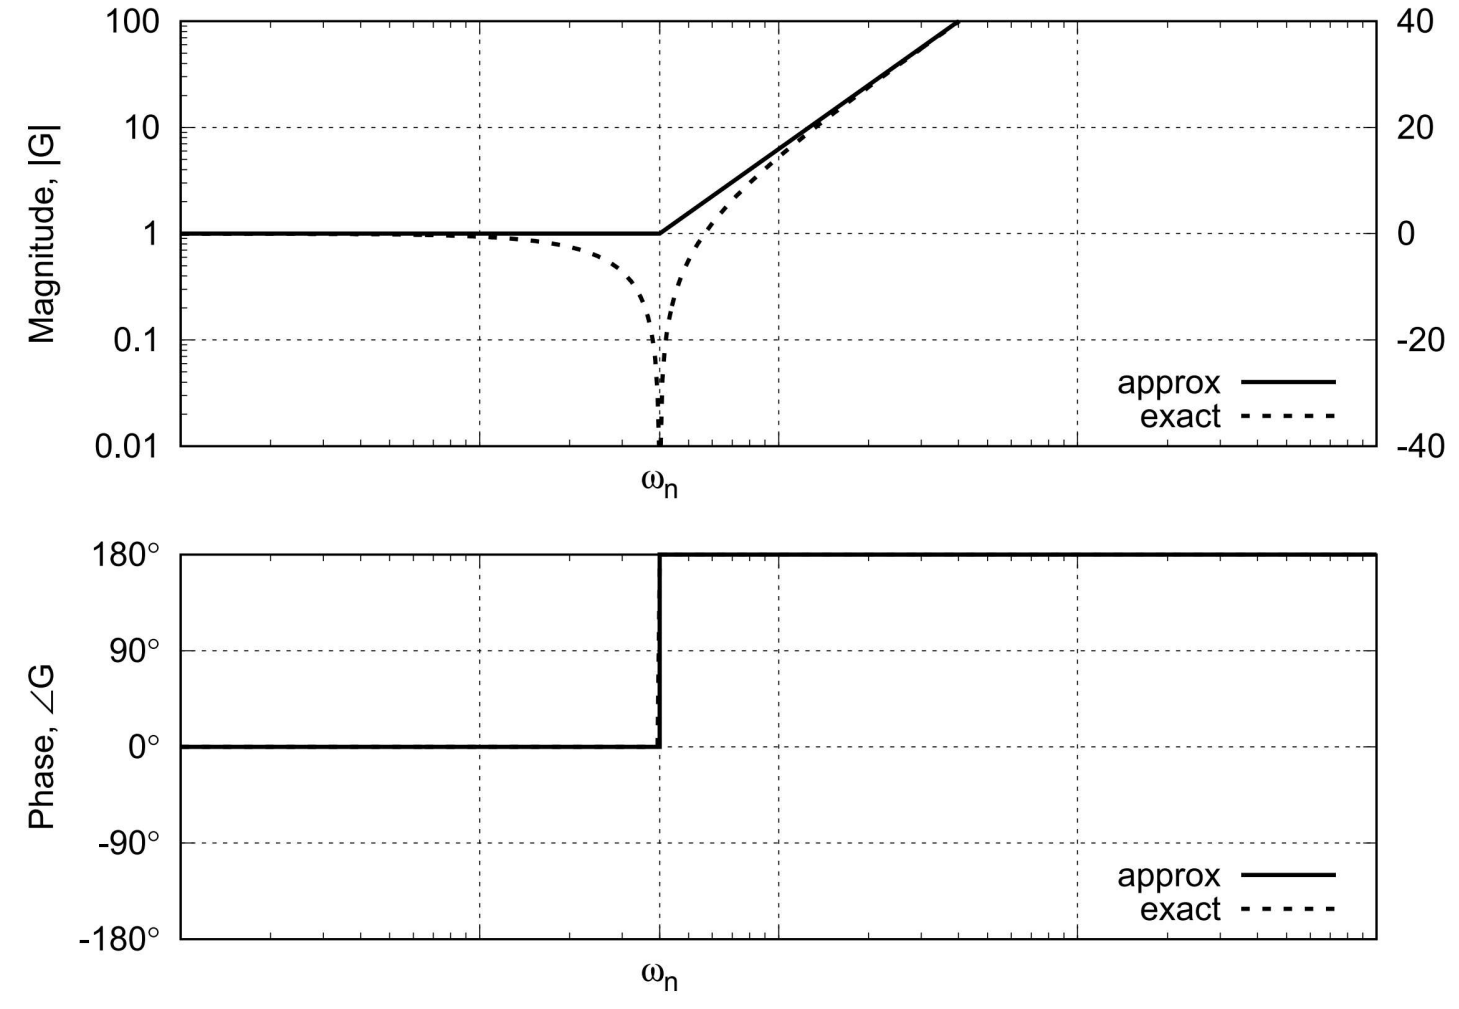
\includegraphics[width=0.6\textwidth]{case8 complex conjucate zero.png}
    \caption{Bode plot for complex conjugate with zero roots of $G(s) = \frac{1}{\omega_{n}^2} 
    (s^2 + \omega_n^2)$, $\omega_n > 0$}
\end{figure}

\subsection{Stability from Bode Plots}
Define two frequencies:
\begin{itemize}
    \item $\omega_{gc}$, gain crossover, is the frequency where the $|G(j\omega)| = 1$.
    \item $\omega_{pc}$, phase crossover, is the frequency where the $\angle G(j\omega) = -180^{\circ}$.
\end{itemize}
The margins can be obtained by
\begin{itemize}
    \item $PM = 180^{\circ} + \angle G(j\omega_{gc})$
    \item $GM = \frac{1}{|G(j\omega_{pc})|}$
\end{itemize}
\begin{figure}[h]
    \centering
    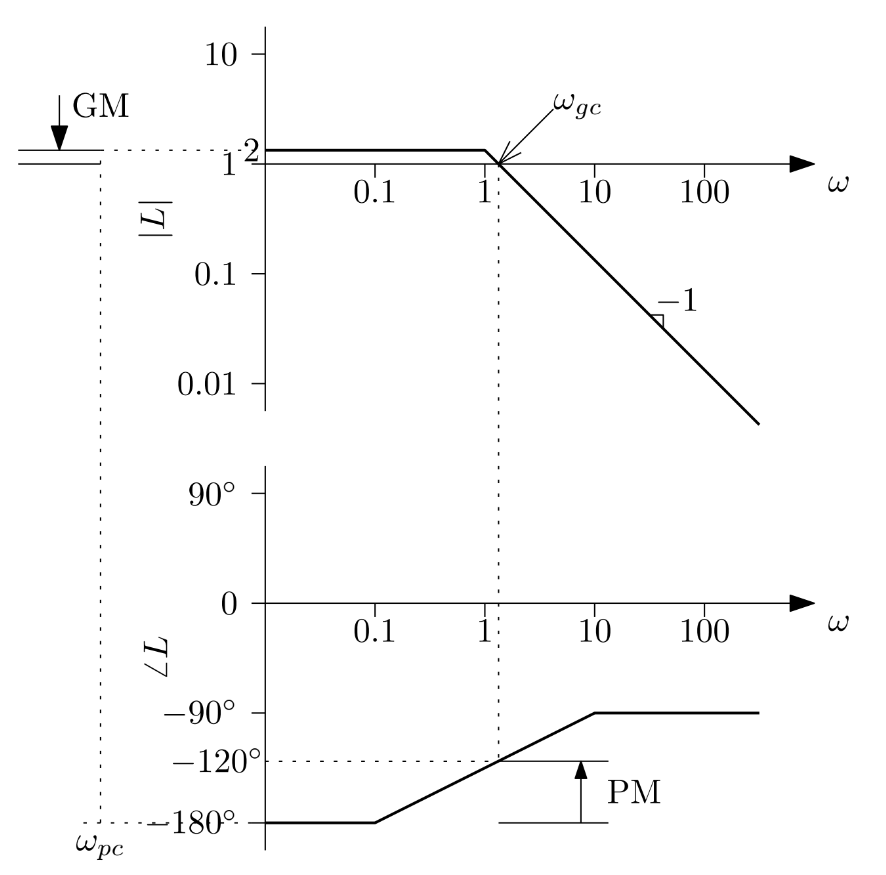
\includegraphics[width=0.6\textwidth]{bode stability diagram.png}
    \caption{Bode plot with margins}
\end{figure}
This can be obtained by
\begin{lstlisting}[language=Matlab]
syms s
G = 1/(s*(s+1)*(s+2));
[n, d] = numden(G);
margin(tf(sym2poly(n), sym2poly(d)))
\end{lstlisting}
right click the graph and select \texttt{Properties $\rightarrow$ Units}, and set to absolute. 

Nyquist margin can be found by considering
\begin{equation*}
    S(s) = \frac{1}{1 + G_p(s) G_c(s)} = \frac{1}{1 + L(s)}
\end{equation*}
and 
\begin{equation*}
    \text{NM} = [\max_{\omega} |S(j\omega)|]^{-1}
\end{equation*}
which can be found easily by
\begin{lstlisting}[language=Matlab]
syms s
L(s) = 1/(s*(s+1)*(s+2));
S(s) = 1/(1 + L(s));
[n, d] = numden(S);
bodemag(tf(sym2poly(n), sym2poly(d)))
\end{lstlisting}

\section{Frequency Response Design}
\subsection{Frequency Response}
The \textbf{frequency response} is the zero-state response $y_{\text{z-s}}(t)$ to $u(t) = \cos\omega t$.

\textbf{Theorem 6.1.1} \textit{Let $G(s)$ be the transfer function of a SISO system. If $G(s)$ is BIBO stable,
i.e. all its poles lie in the open left-hand plane Re($s$)$<0$, the system's frequency response is}
\begin{equation*}
    y_{\text{z-s}}(t) = |G(j\omega)|\cos(\omega t + \angle G(j\omega))
\end{equation*}

Only if $G(s)$ is BIBO stable does a second interpretation of Bode plots hold.
\begin{itemize}
    \item $|G(j\omega)|$ is the magnitude of the frequency response.
    \begin{itemize}
        \item $|G(j\omega)|>1$ is amplification
        \item $|G(j\omega)|<1$ is attenuation
    \end{itemize}
    \item $\angle G(j\omega)$ is the phase of the frequency response.
    \begin{itemize}
        \item $\angle G(j\omega) > 0$ is phase lead
        \item $\angle G(j\omega) < 0$ is phase lag
    \end{itemize}
\end{itemize}

\subsubsection{Frequency Content}
\textbf{Theorem 6.1.2} \textit{Let f(t) be a real-valued signal with an associated Fourier transform}
\begin{equation*}
    F(\omega) = \int_{-\infty}^{\infty} f(t) e^{-j\omega t} dt
\end{equation*}
\textit{where $F(\omega)$ is complex-valued. This signal can be written as}
\begin{equation*}
    f(t) = \frac{1}{\pi} \int_{0}^{\infty} |F(\omega)| \cos(\omega t + \angle F(\omega)) d\omega
\end{equation*}

\subsection{Designing A Frequency Response}'
Define the sensitivity and complementary sensitivity transfer functions:
\begin{align*}
    L(s) &= G_p(s) G_c(s) \\
    S(s) &= \frac{1}{1 + L(s)} \\
    T(s) &= \frac{L(s)}{1 + L(s)} 
\end{align*}
with the identity
\begin{equation*}
    S(s) + T(s) = 1
\end{equation*}
\textbf{Theorem 6.2.1} \textit{
Let $L(s) = G_p(s) G_c(s)$ be the loop transfer function of a closed loop
system, where the product $G_p(s) G_c(s)$ has no pole cancellations in $\text{Re}(s) \geq 0$. This close loop system
is stable if and only if}
\begin{itemize}
    \item \textit{The sensitivity transfer function $S(s) = 1/(1 + L(s))$ is BIBO stable, i.e. has all its poles in $\text{Re}(s) < 0$.}
    \item For each pole $p_k$ of $L(s)$ in $Re(s) \geq 0$ with multiplicity $m_k \geq 1$, 
    \begin{align*}
        S(p_k) = \frac{dS}{ds}(p_k) = ... = \frac{d^{m_k - 1}S}{ds^{m_k - 1}}(p_k) = 0
    \end{align*}
    \item For each zero $z_k$ of $L(s)$ in $Re(s) \geq 0$ with multiplicity $n_k \geq 1$,
    \[
        S(z_k) = 1, \quad \frac{dS}{ds}(z_k) = ... = \frac{d^{n_k - 1}S}{ds^{n_k - 1}}(z_k) = 0
    \]
\end{itemize}
conditions 2 and 3 are known as \textbf{interpolation conditions}.


\section{Matlab Corner}
\subsection{SimplifyFraction}
\begin{lstlisting}[language=Matlab]
syms s
G = (s+1)*(s+2)/(s+3);
simplifyFraction(G)
simplifyFraction(G, 'Expand', true)
\end{lstlisting}
\begin{verbatim}
ans =

((s + 1)*(s + 2))/(s + 3)

ans =

(s^2 + 3*s + 2)/(s + 3)

>> 
\end{verbatim}

\subsection{Root Finding Methods}
\begin{lstlisting}[language=Matlab]
syms s
G = (s+1)*(s+2)/(s+3);
[n, ~] = numden(G);

% Method 1  
c = sym2poly(n);
r = roots(c)

% Method 2
r = solve(n)

% Method 3
r = vpasolve(n)
\end{lstlisting}

\subsection{Nyquist Plot}
\begin{lstlisting}[language=Matlab]
syms s
L = = 1/(s*(s+1)*(s+2));
[n, d] = numden(L);
L = tf(n, d);
nyquist(L)
\end{lstlisting}

\end{document}